\pagenumbering{roman}

\begin{titlepage}
\begin{center}
\ \\

\vspace{15mm}

\large
Charles University in Prague\\
Faculty of Mathematics and Physics\\

\vspace{5mm}

{\Large\bf MASTER THESIS}

\vspace{15mm}


\includegraphics[scale=0.4]{logo.eps} %%% source http://www.mff.cuni.cz/fakulta/symboly/logo.eps

\vspace{20mm}
%\normalsize
{\Large Ondřej Plátek}\\ 

\vspace{5mm}
{\Large\bf Automatic speech recognition using KALDI}

\vspace{20mm}
\large
\noindent
Institute of Formal and Applied Linguistics\\
\noindent
Supervisor: Ing. Mgr. Filip Jurčíček, Ph.D.\\
\noindent
Study branch: Theoretical Computer Science\\
\end{center}
\vspace{20mm}
\begin{center}
Prague 2013
\end{center}

\end{titlepage} % zde koncí úvodní strana

%%%%%%%% 2-3 page with master thesis task
% FIXME -remove this from electronic version%%%%% 
\todon{Insert the task $../images/zadani[1-2].png$ for the printed version}
\newpage
%%%%%%%% end 2-3 page with master thesis task

%%% 4.(2.) title page
\normalsize % nastavení normální velikosti fontu
\vspace{10mm} 

\noindent I would like to thank my supervisor, Ing. Mgr. Filip Jurčíček, Ph.D., for his
advice. \todo{Lorem ipsum dolor sit amet, consectetur adipisicing elit, sed do eiusmod tempor incididunt ut labore et dolore magna aliqua. Ut enim ad minim veniam, quis nostrud exercitation ullamco laboris nisi ut aliquip ex ea commodo consequat. Duis aute irure dolor in reprehenderit in voluptate velit esse cillum dolore eu fugiat nulla pariatur. Excepteur sint occaecat cupidatat non proident, sunt in culpa qui officia deserunt mollit anim id est laborum} 


\vspace{\fill} % nastavuje dynamické umístění následujícího textu do spodní části stránky
\noindent
I declare that I wrote my master thesis independently and exclusively with~the~use of the cited sources. I agree with~lending and publishing this thesis.

%\medskip\noindent
%I acknowledge that my thesis is a~subject to the stipulations of rights and obligations of the Act No. 121/2000 Coll., Copyright Act as valid, especially the~fact that Charles University in~Prague has a right to conclude a~licence agreement on~the use of the~school work as per sect. 60, paragraph 1 of~the~Copyright Act.

\medskip\noindent
I declare that I carried out this master thesis independently, and only with the cited
sources, literature and other professional sources.

I understand that my work relates to the rights and obligations under the Act No.
121/2000 Coll., the Copyright Act, as amended, in particular the fact that the Charles
University in Prague has the right to conclude a license agreement on the use of this
work as a school work pursuant to Section 60 paragraph 1 of the Copyright Act.

\noindent Prague, April 5, 2013 \hspace{\fill}Ondřej Plátek 

%%%   Výtisk pak na tomto míst+ nezapomente PODEPSAT!
%%%                                         *********

%\begin{figure}[htp] \centering{
%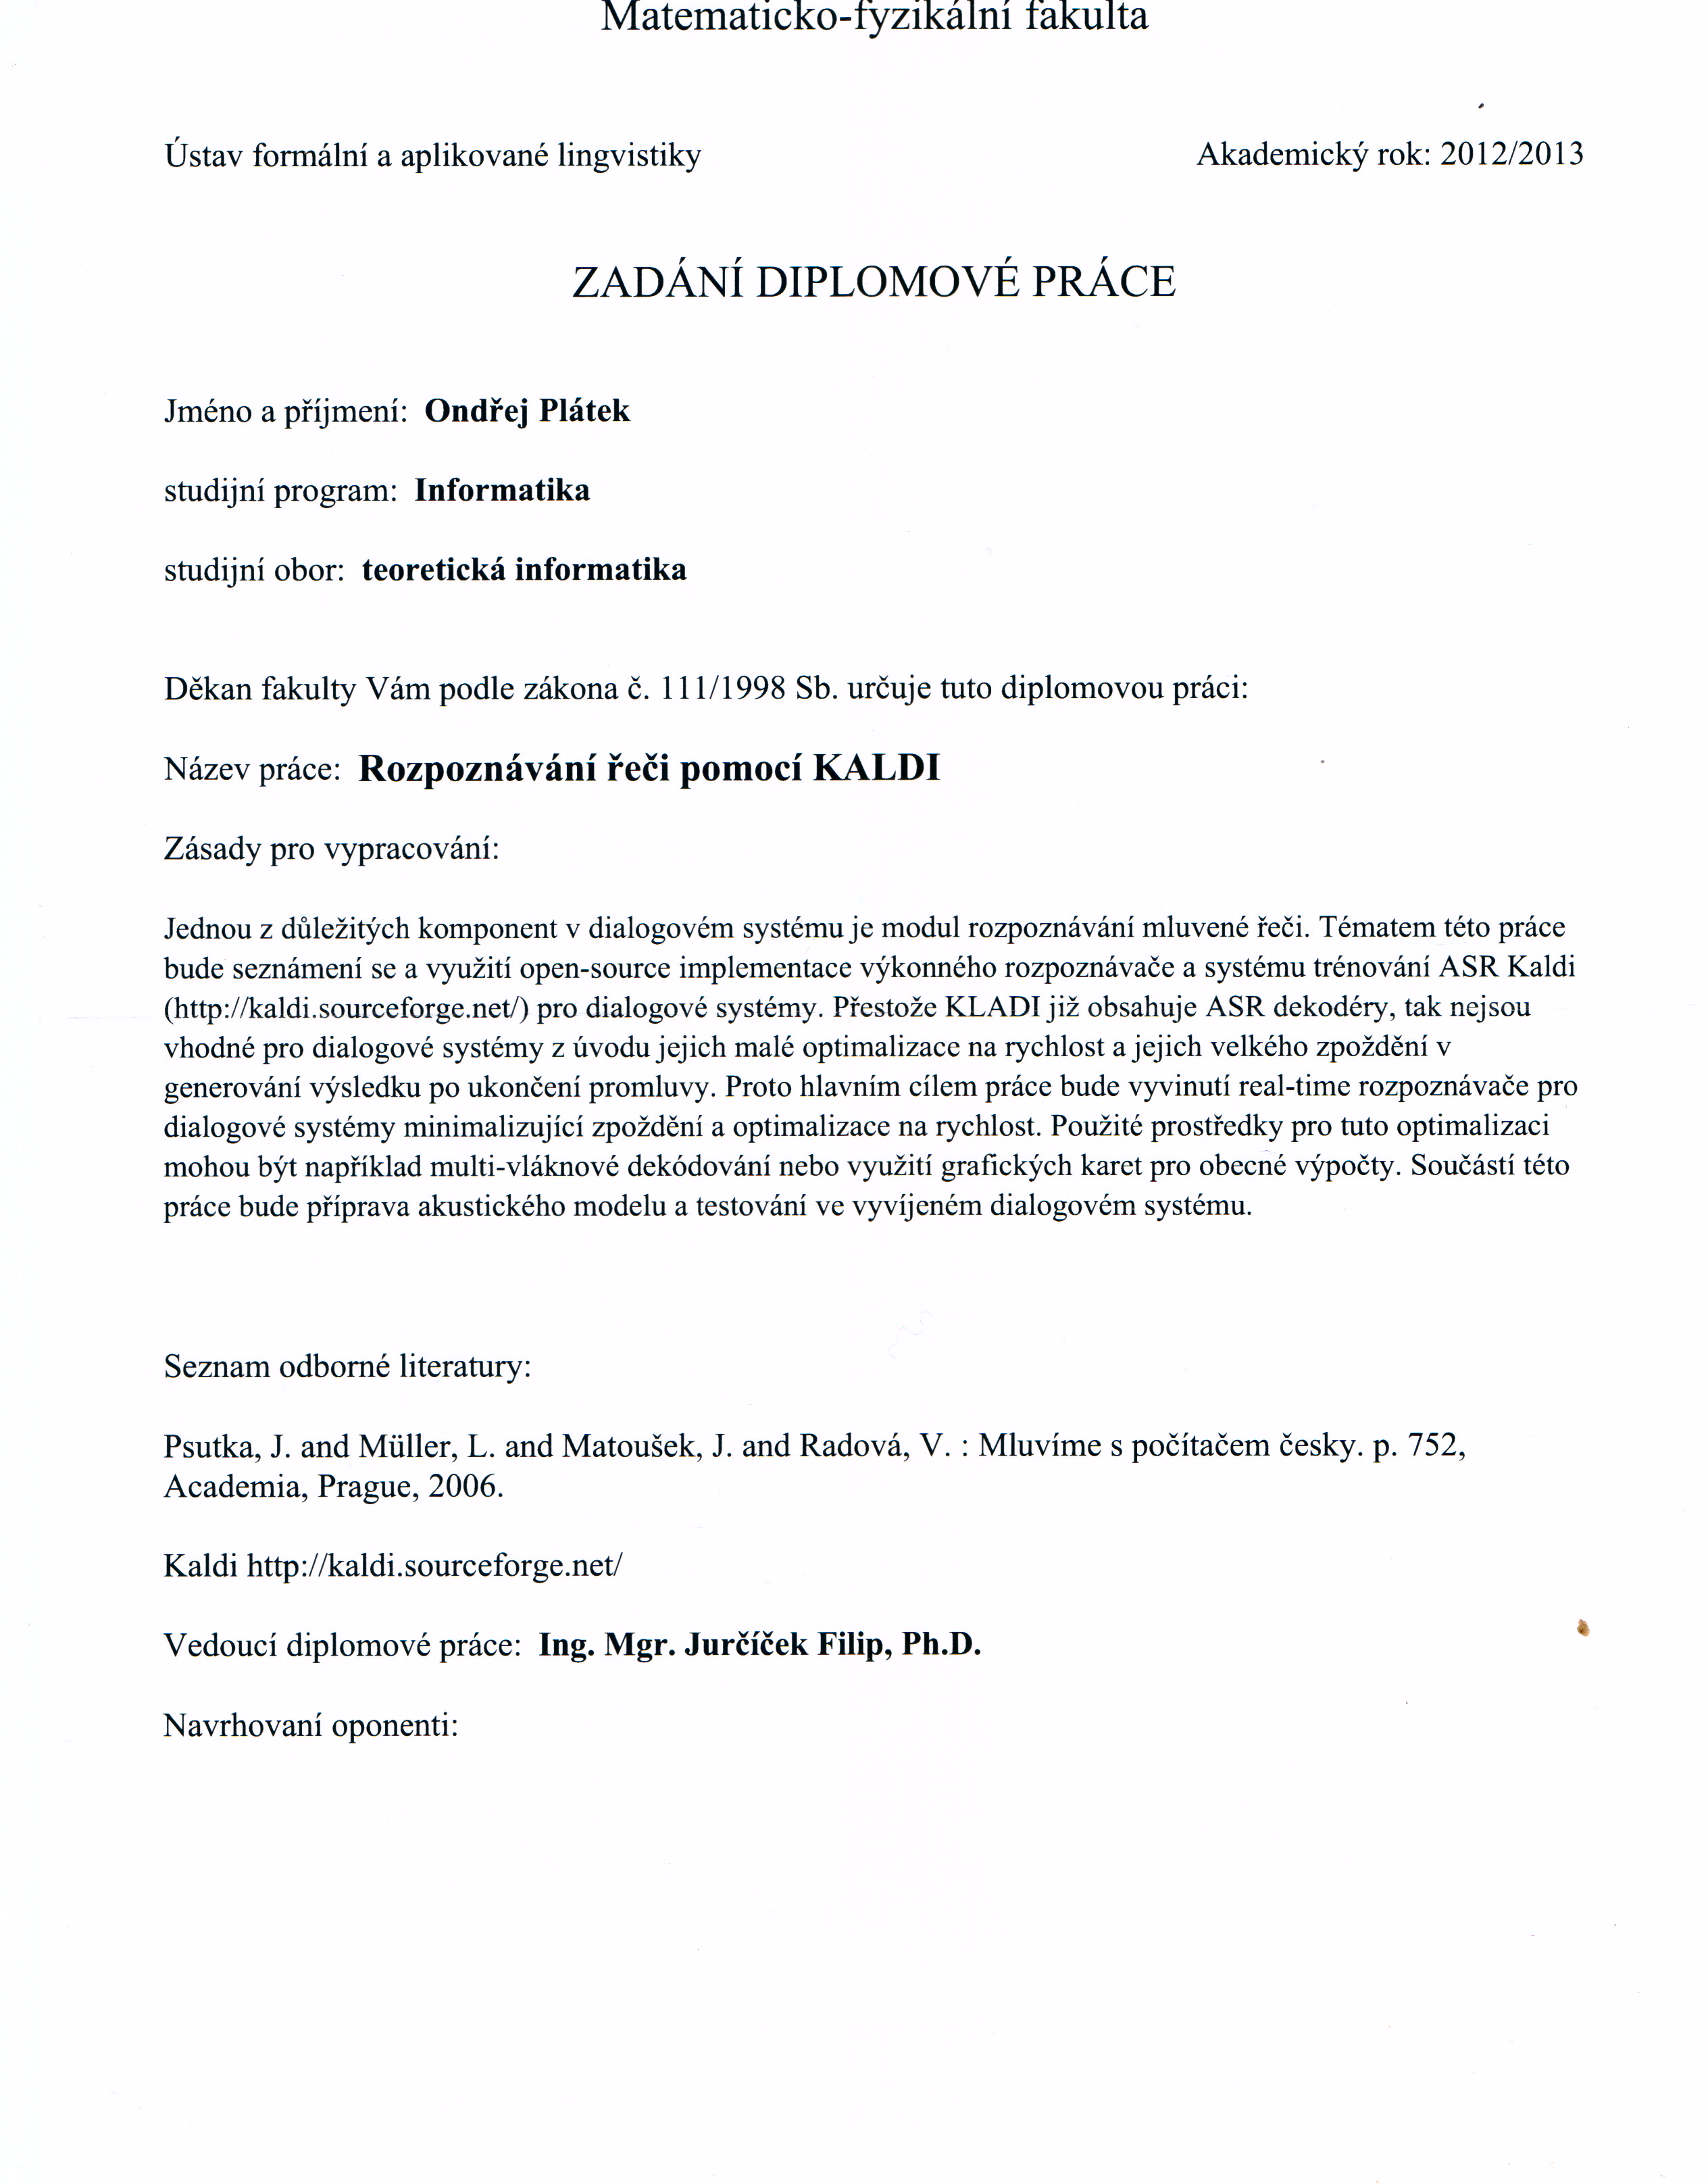
\includegraphics[scale=0.82]{zadani1}}
%\end{figure}  
%
%\newpage
%\begin{figure}[htp] \centering{
%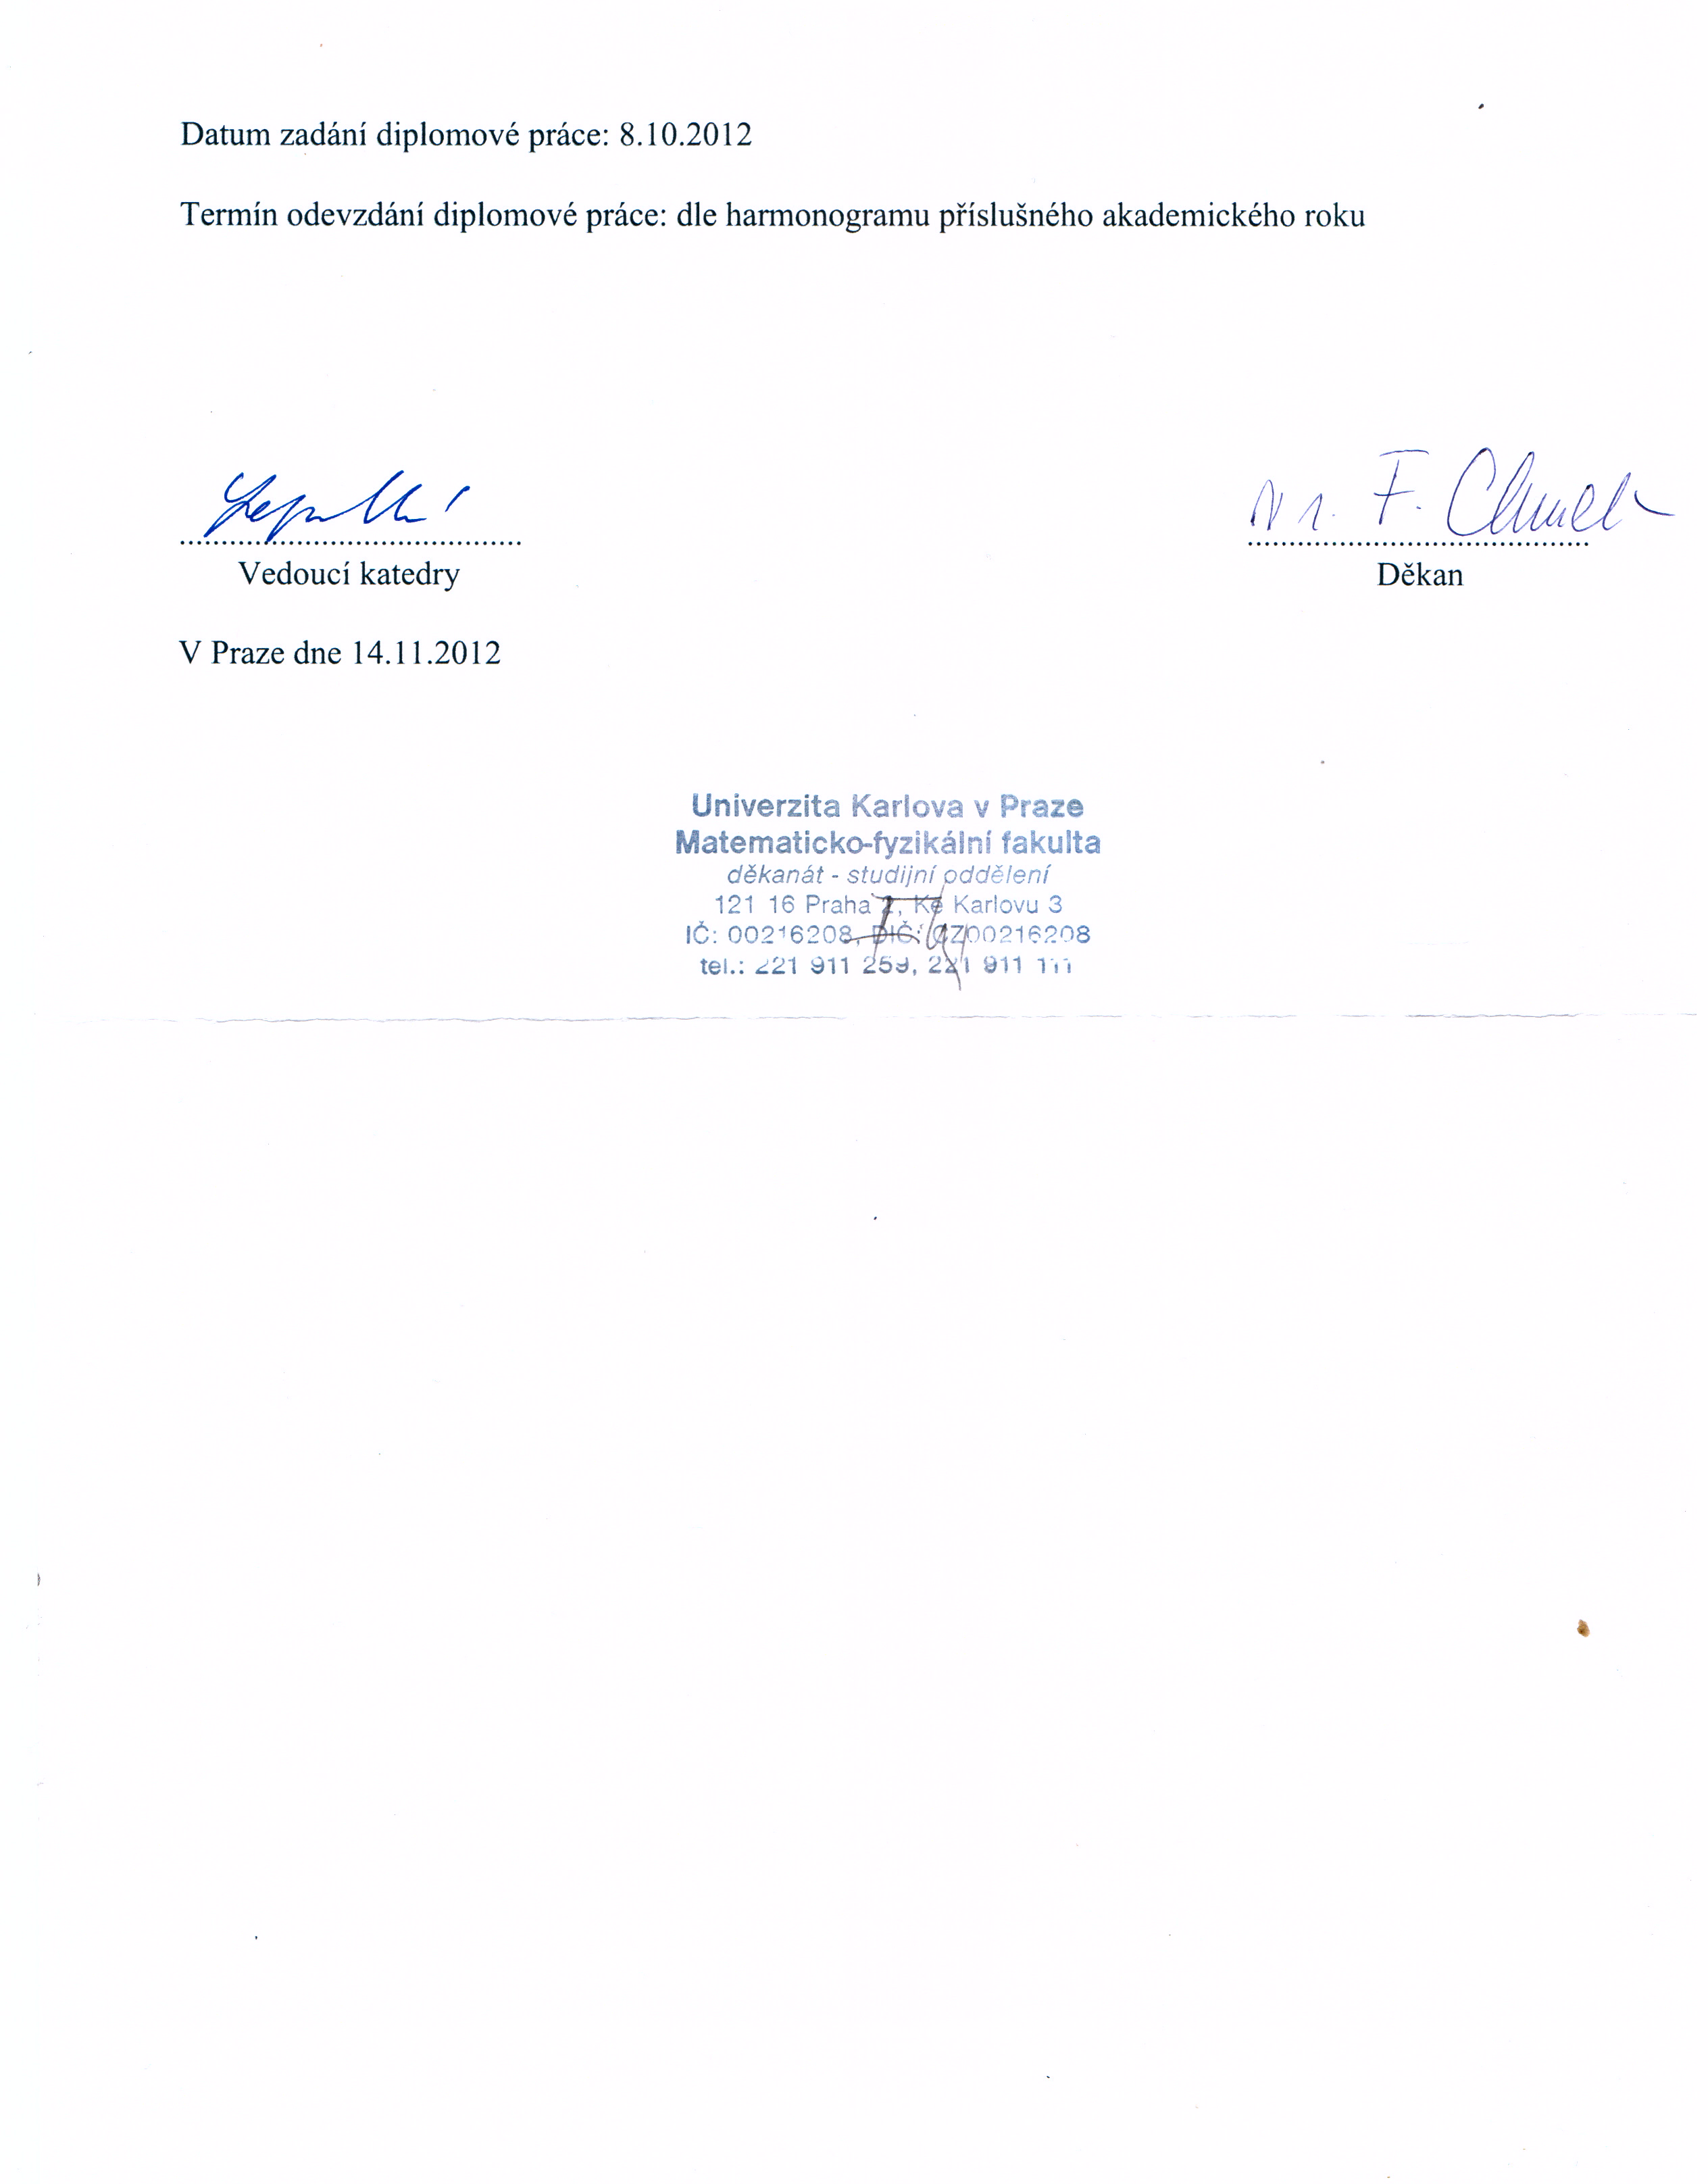
\includegraphics[scale=0.82]{zadani2}}
%\end{figure}  

\newpage

%%% Následuje strana s abstrakty. Doplnte vlastní údaje.
\vbox to 0.5\vsize{
\setlength\parindent{0mm}
\setlength\parskip{5mm}
Název práce: Rozpoznávání řeči pomocí KALDI\\
Autor: Ondřej Plátek\\
Katedra: Ústav formální a aplikované lingvistiky\\
Vedoucí diplomové práce: Ing. Mgr. Filip Jurčíček, Ph.D.\\
e-mail vedoucího: jurcicek@ufal.mff.cuni.cz\\

\noindent Abstrakt:
Jednou z důležitých komponent v dialogovém systému je modul rozpoznávání mluvené řeči. Tématem této práce bude seznámení se a využití open-source implementace výkonného rozpoznávače a systému trénování \\
ASR KALDI (\href{http://kaldi.sourceforge.net/}{http://kaldi.sourceforge.net/})
pro dialogové systémy. 
Přestože KALDI již obsahuje ASR dekodéry, tak nejsou vhodné pro dialogové systémy z úvodu jejich malé optimalizace na rychlost a jejich velkého zpoždění v generování výsledku po ukončení promluvy. Proto hlavním cílem práce bude vyvinutí real-time rozpoznávače pro dialogové systémy minimalizující zpoždění a optimalizace na rychlost. Použité prostředky pro tuto optimalizaci mohou být například multi-vláknové dekódování nebo využití grafických karet pro obecné výpočty. Součástí této práce bude příprava akustického modelu a testování ve vyvíjeném dialogovém systému. 


\noindent Klíčová slova: ASR,rozpoznávání mluvené řeči, dekodér

\vspace{10mm}

\noindent
Title: Automatic speech recognition using KALDI\\
Author: Ondřej Plátek\\
Department: Ústav formální a aplikované lingvistiky \\
Supervisor: Ing. Mgr. Filip Jurčíček, Ph.D.\\
Supervisor's e-mail address: jurcicek@ufal.mff.cuni.cz\\

\noindent Abstract: 
\todo{One of the important compont of a dialog system is a speech recognition module. The topic of this thesis is to use speech recognition training system\\
ASR KALDI (\href{http://kaldi.sourceforge.net/}{http://kaldi.sourceforge.net/}) 
and implement efficient decoder for it. 
KALDI is already deployed with decoders, but they are not convenient for dialog systems, because they are not optimized for speed and they produce results with unbearable delay after utterance finish. The main goal for this thesis is developing real-time decoder for a dialog system, which minimize latency and optimize speed. Suggested methods vary from multi-threading decoding to usage of GPU cards for general computations. Part of this work will be devoted to training of an acoustic model and also testing in real dialog system.
} % end todo

\noindent Keywords: ASR,speech recognition, decoder

\vss}

\newpage

\openright
\pagestyle{plain}
\pagenumbering{arabic}
\setcounter{page}{1}
\tableofcontents


